
%%%%%%%%%%%%%%%%%%%%%%%%%%%%%%%%%%%%%%%%%%%%%%%%%%%%%%%%%%%%%%%%%%%%
\section{Architecture}
\label{sec:architecture}
%%%%%%%%%%%%%%%%%%%%%%%%%%%%%%%%%%%%%%%%%%%%%%%%%%%%%%%%%%%%%%%%%%%%


%%%%%%%%%%%%%%%%%%%%%%%%%%%%%%%%%%%%%%%%%%%%%%%%%%%%%%%%%%%%%%%%%%%%
\subsection{Overview}
\label{sec:architecture_overview}
%%%%%%%%%%%%%%%%%%%%%%%%%%%%%%%%%%%%%%%%%%%%%%%%%%%%%%%%%%%%%%%%%%%%

The framework is divided in to five main concepts as shown in Figure
\ref{fig:architecture}. These are all wrapped into a
\ccc{SimulatorTraits} concept, through which they are accessed to
preform various functions. Users of existing kinetic data structures will need to become familiar with the following two main concepts 
\begin{description}
\item[\ccc{Simulator}] a class that maintains the concept of time and a priority
  queue of the events. It is accessed from the \ccc{SimulationTraits} object using the \ccc{SimulationTraits::simulator_pointer()} method.
\item[\ccc{ActiveObjectsTable}] a container which stores kinetic geometric
  primitives and provides notifications when their trajectories
  change. The \ccc{SimulationTraits} creates an model of this concept
  called \ccc{SimulatorTraits::Moving_point_table} (assuming the
  primitives are points) which is accessible through the
  \ccc{SimulatorTraits::moving_point_table_pointer()} method.
\end{description}
Users who wish to implement kinetic data structures must become
familiar with a further two concepts:
\begin{description}
\item[\ccc{KineticKernel}]  a class which defines kinetic geometric primitives and
  predicates acting on them.
\item[\ccc{InstantaneousKernel}] a model of the CGAL kernel concept which allows static
  algorithms to act on a snapshot of the kinetic data structure.
\end{description}
The final main concept is that of the \ccc{FunctionKernel} a
computational kernel for representing and manipulating functions and
their roots. The \ccc{FunctionKernel}~ is provided by a separate
package and not discussed in detail here (other than the reference
page).

In a typical scenario using the framework, a model of
\ccc{SimulationTraits} is created and a number of geometric primitives
(e.g.\ points) are added to the
\ccc{SimulationTraits::Moving_point_table}. Then a kinetic data
structure, for example a two dimensional kinetic Delaunay
triangulation, is initialized and passed the \ccc{SimulationTraits}
object. The kinetic Delaunay triangulation extracts the trajectories
of the points from the \ccc{SimulationTraits::Moving_point_table} and
the current time from the \ccc{Simulator}. It then uses an instance of
an \ccc{InstantaneousKernel}, obtained from the \ccc{SimulationTraits}
to enable a static algorithm to compute the Delaunay triangulation of
the points at the current time. An instance of a \ccc{Kinetickernel}
is used to compute the \ccc{in_circle} certificate function for each
edge of the initial Delaunay triangulation (in order to verify that
the four points around the edge remain Delaunay). The kinetic data
structure requests that the \ccc{Simulator} solve each certificate
function and schedule an appropriate event. The \ccc{Simulator} uses
the \ccc{FunctionKernel} to compute and compare the roots of the
certificate functions.

Initialization is now complete and the kinetic data structure can be
run. Running consists of the \ccc{Simulator} finding the next event
and processing it until there are no more events. Here, processing an
event involves flipping an edge of the Delaunay triangulation and
computing five new event times (one for each of the edges around the
boundary of the quadralateral containing the edge and one for the edge
being flipped). The processing occurs via a callback from an object
representing an event to the kinetic Delaunay data structure.

If the trajectory of a primitive changes, for example it bounces
off a wall, then the \ccc{ActiveObjectsTable} notifies the kinetic Delaunay data
structure. The kinetic Delaunay data structure then updates all the
certificates of edges adjacent to faces containing the updated point and
reschedules those events with the \ccc{Simulator}.

A more detailed example will be discussed in
Section~\ref{sec:examples}. We will next discuss the main concepts in
order from most fundamental (and least exposed) to most exposed.

\begin{figure*}[htb]
\begin{ccTexOnly}
\begin{center}
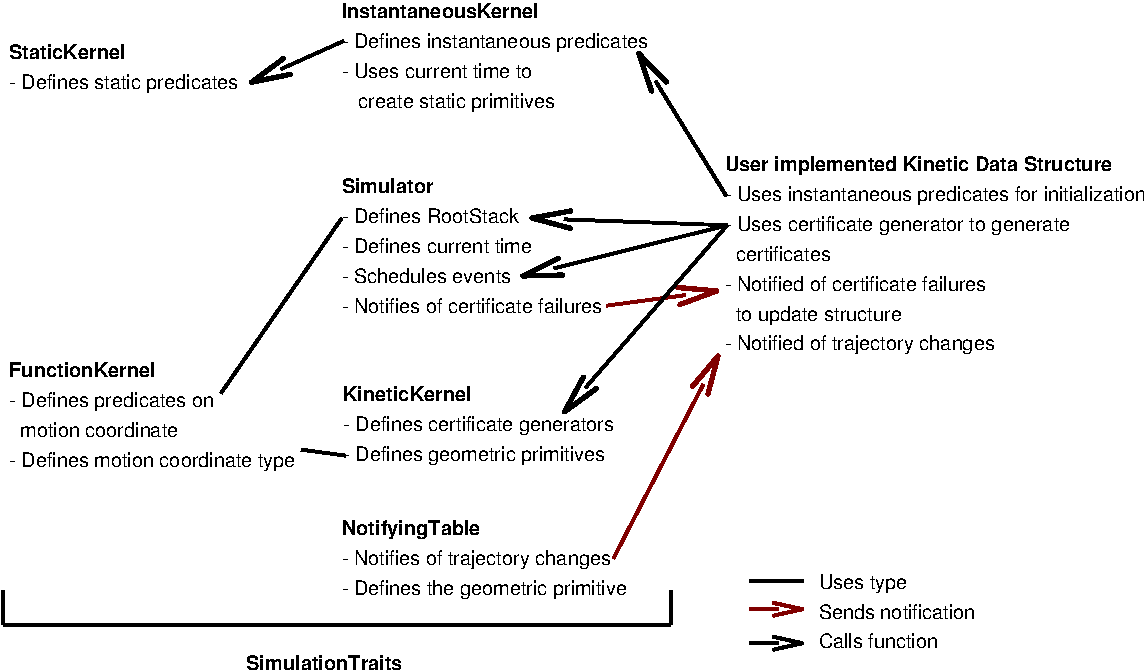
\includegraphics[ scale=.6]{Kinetic_data_structures/architecture_pct}
\end{center}
\end{ccTexOnly}
\begin{ccHtmlOnly}
<img border=1 src="./architecture_pct.gif" align=center alt="The architecture of the kinetic data structures package">
\end{ccHtmlOnly}
\caption{ \label{fig:architecture} 
{\em Framework architecture:} The main concepts and their relationships are shown. }
%\end{minipage}
%\end{center}
\end{figure*}



%%%%%%%%%%%%%%%%%%%%%%%%%%%%%%%%%%%%%%%%%%%%%%%%%%%%%%%%%%%%%%%%%%%%
\subsection{Kinetic primitives and predicates: the KineticKernel.}
\label{sec:kinetic_kernel}
%%%%%%%%%%%%%%%%%%%%%%%%%%%%%%%%%%%%%%%%%%%%%%%%%%%%%%%%%%%%%%%%%%%%

The \ccc{KineticKernel} is the kinetic analog of the CGAL
\ccc{Kernel}. It defines constant complexity kinetic geometric
primitives, kinetic predicates acting on them and constructions from
them. The short example in Section~\ref{sec:architecture_overview}
uses the \ccc{KineticKernel} to compute the \ccc{in\_circle}
certificate functions. We currently provide one model, namely
\ccc{CGAL::KDS::Cartesian_kinetic_kernel<FunctionKernel>}, which
defines two and three dimensional moving weighted and unweighted
points and the predicates necessary for Delaunay triangulations and
regular triangulations. The kernel provides the type \ccc{Function}
which plays the role of the \ccc{RT} in static
CGAL kernels and is the storage type for coordinates of kinetic
primitives. Algorithms request predicate functors from the kernel and
then apply these functors to kinetic primitives.

It is important to note that the \ccc{KineticKernel} does not have any notion of
finding roots of polynomials, of performing operations at the roots of
polynomials, or of static geometric concepts. The first and second are
restricted to the \ccc{FunctionKernel} and the \ccc{Simulator}
(Section~\ref{sec:simulator}). The third is handled by the \ccc{InstantaneousKernel} which
is discussed in the next section.

%%%%%%%%%%%%%%%%%%%%%%%%%%%%%%%%%%%%%%%%%%%%%%%%%%%%%%%%%%%%%%%%%%%%
\subsection{Connecting the kinetic and the static worlds: the InstantaneousKernel.}
\label{sec:instantaneous_kernel}
%%%%%%%%%%%%%%%%%%%%%%%%%%%%%%%%%%%%%%%%%%%%%%%%%%%%%%%%%%%%%%%%%%%%

The \ccc{InstantaneousKernel} allows other CGAL algorithms and data
structures to act on snapshots of a simulation. This ability is useful
for initializing and auditing kinietic data structures. A model of the
\ccc{InstantaneousKernel} concept proves a model of the CGAL
\ccc{Kernel} and works by computing the possition of each primitive in
the snapshot before performing the calculation requested by the static
algorithm.  For example, with the \ccc{InstantaneousKernel} we can use
the \ccc{Delaunay_triangulation_2<Traits, Tds>} to initialize a
kinetic Delaunay data structure and to insert new points into an
existing triangulation. In addition, the \ccc{InstantaneousKernel} can
be used to audit the kinetic data structure by comparing it to the
static data structure computed for that instant in time. We provide
two models, the
\ccc{CGAL::KDS::Cartesian_instantaneous_kernel<ActiveObjectsTable,
Kernel>} and
\ccc{CGAL::KDS::Regular_triangulation_instantaneous_traits<ActiveObjectsTable,
Kernel>}.

We are able to use this technique due to a couple of important
features of the CGAL architecture. First of all, the kernel is stored
as an object in CGAL data structures, so it can have state (for the
\ccc{InstantaneousKernel} the important state is the current time, and
the colection of trajectories). Secondly, predicates are not global
functions, instead they are functors that the algorithm requests from
the kernel. This means that they too, can have internal state. Then,
when an algorithm tries to compute a predicate, the predicate functor
asks the \ccc{InstantaneousKernel} to convert its input (handles to
kinetic geometric primitives) into static primitives and can then use
a predicate from a static CGAL kernel to properly compute the
predicate value.

Note that the time value used by our \ccc{InstantaneousKernel} model
must be support arithmetic operations. Some of the models of
\ccc{FunctionKernel} provide function root types which only support
comparisons, and consequently cannot be used here. In practice, this
is not a severe limitation, as discussed in the next section.

%%%%%%%%%%%%%%%%%%%%%%%%%%%%%%%%%%%%%%%%%%%%%%%%%%%%%%%%%%%%%%%%%%%%
\subsection{Tracking time: the Simulator.}
\label{sec:simulator}
%%%%%%%%%%%%%%%%%%%%%%%%%%%%%%%%%%%%%%%%%%%%%%%%%%%%%%%%%%%%%%%%%%%%

Running a kinetic data structure consists of repeatedly figuring out
when the next event occurs and processing it. This is the job of the
\ccc{Simulator}. It handles all event scheduling, descheduling and
processing and provides objects which can be used to determine when
certificate functions become invalid. Since events occur at the roots
of certificate functions (when the certificate function changes sign),
the \ccc{Root} type defined by a \ccc{FunctionKernel} is used to
represent time by the \ccc{Simulator}. In the example in
Section~\ref{sec:architecture_overview} the kinetic Delaunay data
structure requests that the \ccc{Simulator} determine when
\ccc{in\_circle} certificate functions become invalid and schedules an
\ccc{Event} with the \ccc{Simulator}. When the certificate fails, the
\ccc{Simulator} calls the \ccc{Event::process(Time)} method on the
\ccc{Event}. The framework provides one model of the \ccc{Simulator},
\ccc{CGAL::KDS::Simulator<FunctionKernel, EventQueue>}.

Note that the \ccc{CGAL::KDS::Simulator<FunctionKernel, EventQueue>}
is a object which is accessed by many other objects at run time (for
example, any running kinetic data structures, the graphical
interface). As a result, all access to it is through a reference
counted pointer, \ccc{CGAL::KDS::Simulator<FunctionKernel,
EventQueue>::Pointer}. This pointer can be safely stored. The
\ccc{Simulator} is created by the \ccc{SimulationTraits} and accessed
through the traits.

Our model of the \ccc{Simulator} is parameterized by a
\ccc{FunctionKernel} and a \ccc{EventQueue}. The former allows the
root stack (which allows enumeration of the roots of a polygon) and
root type to be changed, so numeric, exact or filtered exact
computation models can be used. The priority queue is by default a
queue which uses an interface with virtual functions to access the
events, allowing different kinetic data structures to use a single
queue. It can be replaced by a queue specialized for a particular
kinetic data structure if desired.

The \ccc{Root} concept is quite limited in which operations it
supports---it effectively only supports comparisons.  Roots cannot be
used in computations or as the time value in an
\ccc{InstantaneousKernel}. 

Two times, $t_0$ and $t_1$, are considered \textit{topologically
equivalent} if no roots occur in the interval $[t_0,t_1]$. The lack of
separating roots means that the function has the same sign over the
interval. This idea can be extended to a set of kinetic data
structures. When a simulation is running, if the time of the last event
which occurred, $t_{last}$, and the time of the next event,
$t_{next}$, are not equal, then the current combinatorial structures of
all of the kinetic data structures are valid over the entire interval
$(t_{last},t_{next})$. In addition there is a rational value of time,
$t_r$, which is topologically equivalent to all times in the
interval. Computations can be performed at $t_r$ since it can be
easily represented. This flexibility is used extensively in the \ccc{Simulator}.

When such a $t_r$ exists, the kinetic data structures are all
guaranteed to be valid (and the corresponding static data structure
non-degenerate) and so the data structure can be easily audited. The \ccc{Simulator} can
notify the kinetic data structures when this occurs and they can then
use an \ccc{InstantaneousKernel} to perform self-verification.

We can also use this idea to check the correctness of individual
certificates upon construction. We define a certificate to be invalid
when the certificate function is negative. As a result it
is an error, and a common sign of a bug in a kinetic data structure,
to construct a certificate function whose value is negative at the
time of construction. 
%
Unfortunately, the time of construction is
generally a root and this check cannot be performed easily. However,
we can find a time topologically equivalent to the current time for
that function (or discover if no such time exists) and evaluate the
function at that time. This is still a very expensive operation, but
faster than the alternative of using a real number type.

In addition, in order to properly handle two events occurring
simultaneously, the \ccc{Simulator} must check if the certificate function
being solved is zero at the current time. If it is zero, and negative
immediately afterwords, then the certificate fails immediately. This
can be checked in a similar manner.


%%%%%%%%%%%%%%%%%%%%%%%%%%%%%%%%%%%%%%%%%%%%%%%%%%%%%%%%%%%%%%%%%%%%
\subsection{Coordinating many kinetic data structures: the ActiveObjectsTable.}
\label{sec:moving_object_table}
%%%%%%%%%%%%%%%%%%%%%%%%%%%%%%%%%%%%%%%%%%%%%%%%%%%%%%%%%%%%%%%%%%%%

A framework for kinetic data structures needs to support updating the
trajectories of kinetic primitives, such as when a collision occurs,
and notification of the kinetic data structure of such changes. This
requirement is in contrast to static geometric data structures where
the geometric primitives never change and their representations are
often stored internally to the data structure. As a result, primitives
are stored in a centralized table and the data structures stores
\ccc{Key}s instead of the actual primitive. We provide one model of
such a table, \ccc{CGAL::KDS::Active_objects_vector<Object>}.

In the simple example presented in
Section~\ref{sec:architecture_overview}, the kinetic Delaunay
triangulation queries the \ccc{ActiveObjectsTable} for all the moving points on
initialization. Later, when the simulation is running, the
\ccc{ActiveObjectsTable} notifies the kinetic Delaunay data structure whenever a point's
trajectory changes.

More specifically, the \ccc{ActiveObjectsTable} allows multiple kinetic
data structures to access a set of kinetic geometric primitives of a
particular type and alerts the kinetic data structures when a new
primitive is added, one is removed, or a primitive's trajectory
changes. The user must specify what type of kinetic primitive a
particular instance of the \ccc{ActiveObjectsTable} model will contain
through a template argument. This type is exposed as the \ccc{Data}
type shown in the figure. To access an object, a \ccc{Key} which
uniquely identifies the object within this container and which has a
type specific to this container type is used.

The provided models of \ccc{SimulationTraits} each define a model of
\ccc{ActiveObjectsTable} containing points of appropriate
dimensionality. This type is called
\ccc{SimulationTraits::Moving_point_table} and accessed through
\ccc{SimulationTraits::moving_point_table_pointer()}. Like the
\ccc{Simulator} they \ccc{ActiveObjectsTable} models are explicitly shared
and accessed through reference counted pointers.

The \ccc{ActiveObjectsTable} uses a notification system which will be
briefly explained in Section~\ref{sec:misc} to notify interested
kinetic data structures when a set of changes to the primitives is
completed. The kinetic data structures must then request the keys of
the inserted, changed and erase objects from the
\ccc{ActiveObjectsTable} and handle them accordingly. We provide helper
classes to handle a number of common scenarios such as a kinetic data
structure which is incremental and can handle the changes of a single
object at a time (as is done in the example,
Figure~\ref{fig:example_program} in the appendix), or a kinetic data
structure which will rebuild all certificates any time any objects are
changed (which can be more efficient when many objects change at
once). The user can easily add other policies as needed.

The \ccc{ActiveObjectsTable} model provided will not meet the needs of
all users as there are many more specialized scenarios where a more
optimized handling of updates will be needed. The general structure of
the \ccc{ActiveObjectsTable} model can be extended to handle many such
cases. For example, if moving segments are used, then some kinetic
data structures will want to access each segment as an object, where
as others will only need to access the individual endpoints. This extra
capability can be added without forcing any changes to existing (point
based) kinetic data structures by adding methods to return modified
polygons in addition to those which return changed points.

When trajectory changes happen at rational time values, the
\ccc{ActiveObjectsTable} can check that the trajectories are
$C^0$-continuous. Unfortunately, the situation is much more
complicated for changes which occur at roots. In practice, motions can
be rounded off to nearby rational values without problem.

The \ccc{ActiveObjectsTable} only knows about one type of kinetic
primitive and has no concept of time, other kinetic primitives or
predicates. When a kinetic data structure handles an insertion, for
example, it must query the \ccc{Simulator} for an appropriate time
value and generate primitives using the \ccc{KineticKernel}. A more
detailed discussion of how to use the \ccc{ActiveObjectsTable} appears
in Section~\ref{sec:examples}.

%%%%%%%%%%%%%%%%%%%%%%%%%%%%%%%%%%%%%%%%%%%%%%%%%%%%%%%%%%%%%%%%%%%%
\subsection{Miscellaneous: graphical display, notification and reference management.}
\label{sec:misc}
%%%%%%%%%%%%%%%%%%%%%%%%%%%%%%%%%%%%%%%%%%%%%%%%%%%%%%%%%%%%%%%%%%%%

We describe some coding conventions used, graphical display,
notification and reference management support in the framework in the
following sections.


\subsubsection{Graphical display}

We provide a number of different classes to facilitate graphical
display and manipulation of kinetic data structures. There are two and
three dimensional user interfaces based on the Qt
(\ccc{CGAL::KDS::Qt_widget_2<Simulator>}) and Coin (\texttt{http://www.coin3d.org})
(\ccc{CGAL::KDS::QT_widget_3<Simulator>}) libraries,
respectively.  The graphical interfaces allows the simulations to be
start and stopped, events can be stepped through and time reversed.

We provide support for displaying two and three dimensional weighted
and unweighted point sets and two and three dimensional CGAL
triangulations. Other types can be easily added.

\subsubsection{Reference management}

A number of objects need to maintain pointers to other independent
objects. For example, each kinetic data structure must have access to
the \ccc{Simulator} so that it can schedule and deschedule events. These
pointers are all reference counted in order to guarantee that they are
always valid. We provide a standard reference counting pointer and
object base to facilitate this, namely \ccc{Ref_counted<Object>}.

Each shared object in the framework defines a type \ccc{Pointer} which is the
type for a reference counter pointer pointing to it. These should be
used for storing pointers to the objects in order to avoid dangling
pointers. In addition, many of the objects expect such pointers as
arguments.

\subsubsection{Runtime event passing}

Runtime events must be passed from \textit{notifiers}, namely the
\ccc{ActiveObjectsTable} and the \ccc{Simulator} to the kinetic data
structures to \textit{listeners}, such as a kinetic data structure
which needs to update itself when an event occurs These are passed
using a simple, standardized notification interface. To use
notifications, first defines a small proxy class which inherits from a
\ccc{Listener} base type provided by the notifier. The \ccc{Listener}
base class registers itself with the notifier on construction (and
unregisters itself on destruction).

When the some state of the notifier changes it, it calls the
\ccc{new_notification} method on the proxy object provided and passes
it a label corresponding to the name of the field that changed. The
proxy object can then call an appropriate method on the kinetic data
structure or other listening class.

In order to unregister on destruction, the \ccc{Listener} must store a
(reference counted) pointer to the object providing
notifications. This pointer can be accessed through the \ccc{notifier}
field. The \ccc{Listener} object stores a reference counted pointer to
the notifying object, while the notifying object stores a plain
pointer to the \ccc{Listener}. It can do this since the \ccc{Listener}
is guaranteed to unregister itself when it is destroyed. This avoids
circular reference counted pointers.

